\chapter{RANSAC based linear feature Extraction}

\section{Overview}

In indoor environments on of the most ubiquitous features are walls. There maybe other features and obstacles to avoid and plan a path around, but it is essential you first map the walls so that you know where you are. In this implementation we use the LIDAR described in chapter \ref{cha:Platform} to find walls in our environment. We do this using a RANSAC based algorithm, which is also robust to people and other obstacles in the environment\cite{}. Once we have the walls we need to derive the measurement model for how a wall like linear feature is used in EKF SLAM. It is obvious that the measurement model and it's derivatives will not be the same as in point features as the wall moves very differently as the robot moves. For example it is not possible to know the robot's motion from the previous motion model if the robot is moving along a wall. Hence we need different measurement models and derivatives. 

\section{Feature Extraction Algorithm}

For linear features we are essentially trying to fit a line or multiple lines onto a set of points. There are a large number of methods to do that such as least squares, Split-merge and RANSAC\cite{}. Looking into a few implementations of RANSAC in common libraries such as PCL and OpenCV, we see that it tries to robustly fit a line to the given set of points. In regular environments, since more than one wall can be seen at a time, it becomes necessary to first segment the data before using the algorithm. Instead another approach is to randomly sample points and try to fit multiple lines simultaneously. This   is explained in algorithm \ref{alg: RANSAC algorithm}\cite{}.

\begin{algorithm}[H]
\begin{algorithmic}

	\While{
	\begin{itemize}
		\item there are still unassociated laser readings, 
		\item and the number of readings is larger than the consensus, 
		\item and we have done less than N trials.
	\end{itemize}
	}
	\begin{itemize}
	\item Select a random laser data reading. 
	\item Randomly sample S data readings within D degrees of this laser 
	data reading 
	\item Using these S samples and the original reading calculate a 
	least squares best fit line. 
	\item Determine how many laser data readings lie within X distance 
	from this best fit line
	\item If the number of laser data readings on the line is above some 
	consensus C do the following: 
		\begin{itemize}
			\item calculate new least squares best fit line based on all 
			the laser readings determined to lie on the old best fit 
			line. 
			\item Add this best fit line to the lines we have extracted. 
			\item Remove the number of readings lying on the line from the 
			total set of unassociated readings.
		\end{itemize}
	\end{itemize}
	\EndWhile
\end{algorithmic}
	\caption{Multiple line fitting with RANSAC}
	\label{alg: RANSAC algorithm}
\end{algorithm}

As it is seen in the algorithm, we only extract lines and not line segments. Hence all lines are assumed to be infinite. While this is not actually true in most environments it is a good approximation for relatively long line segments which model walls.


\section{Measurement Model and the corresponding differentials}
\label{sec:Ransac_math}
Once the lines in the data are recovered, we need an effective representation to store them. The common, slope-point form has a major disadvantage when trying to represent perfectly vertical lines and the two point form will expand the size of the measurement vector $ z $ increasing the calculation required for \ekf. So it is preferable to represent it in the normal form where, just the coordinates of the point of intersection of the normal from the origin to the line is stored. For example, in figure \ref{fig: normal_form} the line can be represented solely by the point $ D $.

\begin{figure}
\centering
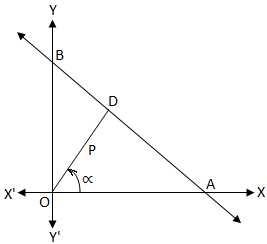
\includegraphics[width=0.3\textwidth]{normal_form}
\caption{Normal form of a line}
\label{fig: normal_form}
\end{figure}

Once we have a line, we need to convert it to the inertial frame of reference as in section \ref{sec:Spike_math}. Unlike point features we are not trying to find the same point in a different frame but the same line. In figure \ref{fig: wall_to_world} we have point $ P_1 $ in robot frame and we need to find point $ P_2 $ in inertial given coordinates of the robot in inertial frame as $ P_r $. For which we use Algorithm \ref{alg: wall_to_world}.
\begin{figure}
\centering
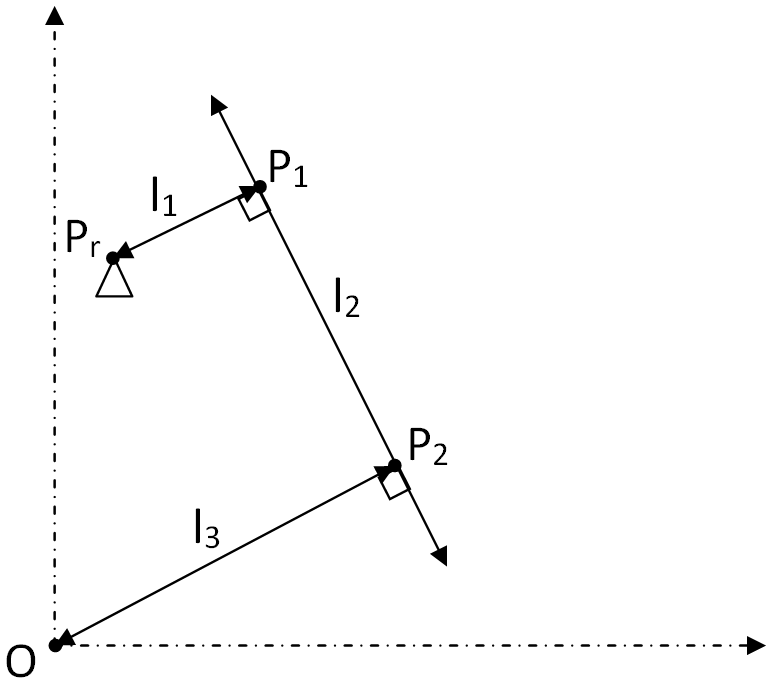
\includegraphics[width=0.3\textwidth]{wall_to_world}
\caption{Line in robot frame and world frame.}
\label{fig: wall_to_world}
\end{figure}

\begin{algorithm}
	\begin{enumerate}
		\item Convert point $ P_1 $ from robot frame of reference to inertial frame as in section \ref{sec:Spike_math}
		\item Given points $ P_r $ and $ P_1 $ in inertial frame, the equation of line $ l_1 $ is found using two point form of a line
		\item Since $ l1 \perp l2 $ the slope of $ l_2 $ is the negative reciprocal of the slope of $ l_1 $. 
		\item Using the slope and the point $ P_1 $ the equation of line $ l_2 $ is found using slope-point form of a line.
		\item The equation of line l3 is found similarly using slope of $ l_1 $ and point $ O $. 
		\item Solving equations for $ l_3 $ and $ l_2 $ we get the coordinates of point $ P_2 $. 
	\end{enumerate}
\caption{To convert linear features from robot frame to inertial frame}
\label{alg: wall_to_world}
\end{algorithm}

Once we have the landmark in the world frame we need to see if it corresponds to any existing landmark in the map. We check this by comparing both the perpendicular distances between the walls and the angle between the walls. This allows us to have 2 tuning parameters so that the association can be weighted as desired. Usually since most walls in an indoor environments are at right angles, the variation allowed in angle for the association is larger compared to distance. 

Algorithm \ref{alg: wall_to_world} is also called the inverse measurement model as in subsequent time steps for the measurement model we do the exact opposite process. That is given a line using it's normal form in inertial frame, we need to get the \textit{measurement} from the robot. That is, we need the perpendicular distance from the robot to the wall and the angle of the laser beam which would hit the wall normally. For this given coordinate pf point $ P_2 $ as $ (x_2,y_2) $ and the robot pose as $ (x_r,y_r,\theta_r) $ we get $ P_1 $ using equation \ref{eq:lineModel1}. 

\begin{equation}
	\label{eq:lineModel1}
	x_1 = x_2 - \frac{y_2 ( x_2 y_ r- y_2 x_r)}{(x_2^2 + y_2^2)}
	\qquad
	y_1 = y_2 + \frac{x_2 ( x_2 y_ r- y_2 x_r)}{(x_2^2 + y_2^2)}
\end{equation}

\begin{equation}
	\label{eq:lineModel2}
	r=\sqrt{(y_1-y_r)^2+(x_1-x_r)^2}
	\qquad
	\alpha = \tan^{-1}\left(\frac{y_1-y_r}{x_1-x_r}\right)-\theta_r
\end{equation}

Once we have $ P_1 $, we can find the perpendicular distance $ r $ and angle $ \alpha $ using equation \ref{eq:lineModel2} giving measurement model $ h $ as per equation \ref{eq:lineModel3}. This measurement can be used to calculate the \textit{innovation} as per equation \ref{eq:EKF_8}. 

\begin{equation}
	\label{eq:lineModel3}
	h=\begin{bmatrix}
	r\\\alpha
	\end{bmatrix}
\end{equation}

For calculating the \textit{Kalman Gain}, we need the Jacobian matrix $ H $. As each wall is independent of the other, this has the same structure as explained in section \ref{sec:Spike_math} and is given by equation \ref{eq:SpikeMath3}. We derive each of the terms separately as per equation \ref{eq:lineModel5} and \ref{eq:lineModel6}.  

\begin{subequations}
\label{eq:lineModel5}
	\begin{align}
	\beta &= \frac{x_rx_1-x_1^2-y_1^2+y_ry_1}{x_1^2+y_1^2}\\
	\frac{\partial r}{\partial x_r} &= 2x_1\beta \quad
	\frac{\partial r}{\partial x_r} = 2y_1\beta \quad
	\frac{\partial r}{\partial \theta_r} = 0 \\
	\frac{\partial \alpha}{\partial x_r} &= 0 \quad 
	\frac{\partial \alpha}{\partial y_r} = 0 \quad 
	\frac{\partial \alpha}{\partial \theta_r} = -1
	\end{align}
\end{subequations}

\begin{subequations}
\label{eq:lineModel6}
	\begin{align}	
	\gamma &= \frac{x_rx_1-x_1^2-y_1^2+y_ry_1}{x_1^2+y_1^2} \\
	\frac{\partial r}{\partial x_1} &= 
	-2x_1\gamma^2 - 2\gamma(2x_1-x_r) \\
	\frac{\partial r}{\partial y_1} &= 
	-2y_1\gamma^2 - 2\gamma(2y_1-y_r)	\\
	\frac{\partial \alpha}{\partial x_1} &=  \frac{-y_1}{x_1^2+y_1^2}\qquad
	\frac{\partial \alpha}{\partial y_1} =
	\frac{x_1}{x_1^2+y_1^2} 
	\end{align}
\end{subequations}

Having the Jacobian matrices we can use the same observer error given by equation \ref{eq:SpikeMath5} to correct the position estimate using equations \ref{eq:EKF_7} to \ref{eq:EKF_9}.

\section{Experimental results}
\textit{Description of the arena and the run performed.}

\textit{Images of the path ground truth and correction.}

We see that it estimates the path taken by the robot to a good extant as well as gives us a better idea of the environment. As walls are an ubiquitous feature found in most indoor environments, this representation gives us more information. But it is very slow. 
 